\documentclass[12pt]{article}
\usepackage{amsmath}
\usepackage{graphicx}
\usepackage{cite}
\usepackage{hyperref}
\usepackage{authblk}

\title{Document Similarity for Low Energy Nuclear Reactions}
\author[1]{Anasse Bari}
\author[1]{Atmaj Koppikar}
\author[1]{Tanya Pushkin Garg}
\author[1]{Yvonne Wu}
\author[2]{David J. Nagel}
\affil[1]{Courant Institute of Mathematical Sciences, New York University, New York, NY, United States}
\affil[2]{School of Engineering and Applied Science, George Washington University, Washington, DC, United States}
\affil[ ]{\texttt{abari@nyu.edu}}

\date{February 16, 2025}

\begin{document}

\maketitle

\begin{abstract}
    The urgent global demand for clean energy solutions has intensified research into Low Energy Nuclear Reactions (LENR), a promising field for sustainable energy production.
     While prior work focused on analyzing LENR abstracts using topic modeling and a two-phase clustering approach, this study advances the field by developing a full-text document similarity framework that addresses structural variability in scientific literature. 
     We introduce a novel grouping-based method that divides documents into three semantically coherent chunks, aggregates their embeddings via arithmetic averaging, and computes similarity through localized group-wise comparisons. 
     Leveraging OpenAI embeddings and Milvus vector storage, our approach achieves a higher similarity score and reduces query latency to a 4× improvement over the previous two-phase algorithm. 
     While the narrowed semantic focus lowers topic diversity (0.0194 vs. 0.98 previously), comprehensive evaluation across 3,424 documents reveals robust scalability and efficient handling of heterogeneous formats (journal articles, technical reports, multilingual content). The system demonstrates a 0.2315 average cosine similarity when evaluated corpus-wide, reflecting its capacity to identify nuanced connections across diverse LENR studies. 
     We deploy these advancements in an open-access tool that enables researchers to efficiently retrieve semantically similar studies through an intuitive dashboard.
     This work bridges critical gaps in nuclear energy literature analysis, offering a blueprint for AI-driven discovery in complex scientific domains.
\end{abstract}

\textbf{Keywords}: Low Energy Nuclear Reactions (LENR), Nuclear Energy, Predictive Analytics, Artificial Intelligence, Unsupervised Learning.

\section{Introduction}
The global energy crisis, driven by population growth and climate change, demands urgent innovation in clean energy technologies. Among emerging solutions, Low Energy Nuclear Reactions (LENR) stand out for their potential to enable safe, scalable nuclear energy production at ambient temperatures. Unlike traditional nuclear fission, LENR systems exhibit minimal radiation byproducts and utilize abundant isotopes like deuterium, offering a path toward sustainable energy independence1. However, progress in this field has been hindered by the fragmented nature of LENR research—spanning 3,424 documents across 34 years in formats ranging from conference abstracts to technical reports in multiple languages.
Prior efforts to analyze LENR literature, including our own work2, focused narrowly on abstracts using clustering algorithms like BERTopic. While effective for identifying high-level themes, this approach overlooks critical technical details embedded in full-text documents—a limitation compounded by the structural heterogeneity of LENR papers (e.g., inconsistent section headers, embedded equations, and multilingual content).
This paper introduces an AI-driven framework that overcomes these challenges through three innovations:
Full-text semantic analysis: Leveraging OpenAI’s text-embedding-3-small embeddings to capture nuanced relationships across entire documents, not just abstracts.
Adaptive chunking: Dividing documents into three context-preserving groups using 512-token segments with 20\% overlap, enabling localized similarity comparisons while accommodating structural variability.
% Milvus-optimized retrieval: Implementing a hybrid IVF_FLAT index that achieves query latency—4 times faster than prior two-phase clustering approaches—while maintaining a coherence score of 0.5578 (vs. 0.14 for BERTopic methods).
    
    \section{Background and Related Work}

    Document similarity is a critical task in information retrieval, enabling effective organization, clustering, and retrieval of relevant documents. Various approaches have been developed to compute document similarity, ranging from traditional methods like cosine similarity with TF-IDF to advanced neural network-based embeddings. This section reviews the previous work on LENR document similarity, discusses aspect-based similarity approaches, and highlights challenges posed by varying document lengths and formats.
    
    \subsection{LENR Document Similarity using abstracts}
    
    The previous study on Low Energy Nuclear Reactions (LENR) by Bari et al. \cite{bari2024exploring} introduced a machine learning tool for identifying similar research studies. The tool relied on topic modeling techniques such as Latent Dirichlet Allocation (LDA), BERTopic, and Top2Vec to uncover latent themes in LENR abstracts. The proposed two-phase algorithm utilized BERTopic clusters to narrow down the search space before computing cosine similarity between query documents and documents within the selected cluster.
    
    However, the previous system was limited to analyzing only the abstracts of LENR research papers. While abstracts provide concise summaries of research, they often lack the depth and context present in full-text documents. This limitation restricted the tool's ability to capture nuanced semantic relationships across the entire corpus. In contrast, our updated system processes full-text documents, leveraging embeddings generated from all sections of a paper to provide a more comprehensive understanding of document similarity.
    
    \subsection{Aspect-Based Document Similarity}
    
    Aspect-based document similarity extends traditional similarity measures by incorporating specific aspects of documents, such as methodology or findings \cite{ostendorff2020aspect}. For instance, Ostendorff et al. \cite{ostendorff2020aspect} proposed an aspect-based approach for research papers using Transformer models like SciBERT and RoBERTa. Their method involved pairwise classification tasks where citations were used as labels to identify specific aspects of similarity between documents.
    
    While aspect-based approaches offer fine-grained comparisons, they rely heavily on consistent document structure and labeled data for training. In the case of LENR research papers, which vary widely in structure and content format (e.g., journal articles, conference presentations, white papers), such methods are impractical. The lack of consistent section titles or labeled aspect data makes it challenging to apply aspect-based techniques effectively in this domain.
    
    \subsection{Document Similarity with Varying Lengths}
    
    Measuring similarity between documents of varying lengths poses unique challenges due to differences in lexical density, abstraction levels, and contextual richness. Gong et al. \cite{gong2018hidden} addressed this issue by comparing texts in a common space of hidden topics using topic modeling techniques. Their approach demonstrated robust performance in aligning long documents with their concise summaries.
    
    Similarly, Ostendorff et al. \cite{ostendorff2022specialized} proposed specialized embeddings for aspect-based similarity that scale linearly with corpus size while preserving coherence across varying document lengths. These methods highlight the importance of designing representations that bridge lexical and contextual gaps between long-form texts and shorter summaries.
    
    In our study, we adopt a grouping-based approach inspired by these works but tailored to handle the inconsistent structure of LENR documents. By dividing each document into equal-sized groups of chunks and aggregating their embeddings, we ensure that semantic information is preserved while accommodating variations in length and format.
    
    \subsection{Limitations of Existing Approaches}
    
    Traditional methods like cosine similarity with TF-IDF \cite{kdnuggets2025evaluating} fail to capture semantic nuances across documents with differing lengths or structures. While neural embedding models such as BERT \cite{devlin2019bert} and SciBERT \cite{beltagy2019scibert} offer improved contextual understanding, their effectiveness diminishes when applied without preprocessing strategies tailored to domain-specific challenges.
    
    Aspect-based methods \cite{ostendorff2020aspect} provide granularity but require consistent structural features or labeled data for training. These requirements are unmet in the LENR corpus due to its diverse formats and lack of standardized sectioning.
    
    Our grouping approach addresses these limitations by:
    \begin{itemize}
        \item Splitting documents into manageable chunks based on token count.
        \item Aggregating chunk embeddings into group-level representations.
        \item Comparing groups using cosine similarity to capture localized semantic relationships.
    \end{itemize}
    
    This method balances computational efficiency with semantic richness, making it suitable for analyzing large-scale corpora like LENR.
    % -------------------------------------
\section{Dataset}
    This study uses a comprehensive LENR bibliography hosted by Rothwell (2002), with over 4,743 entries, including metadata like titles, abstracts, and authors. The dataset is further expanded by manually collecting additional documents, providing a robust corpus for analysis.

\subsection{Nature of the LENR Dataset}
The LENR corpus comprises 3,424 documents collected from scientific publications, conference proceedings, technical reports, and white papers spanning 1989-2023. 
This heterogeneous collection of Multilingual content, Format inconsistencies and Structural variability presents unique challenges:

\subsection{PDF Processing with GROBID}
We employed GROBID (GeneRation Of BIbliographic Data) to extract structured content from raw PDFs through its machine learning-powered pipeline. The header extraction process identified titles, authors, and affiliations with 92\% accuracy (F1-score). Content segmentation divided documents into hierarchical sections such as abstract, methodology, and results using CRF models. Metadata enrichment extracted references, figures, and equations as TEI-XML elements. Text normalization converted special characters (e.g., LaTeX equations to Unicode) and standardized whitespace. The processed output was stored in a database.

\subsection{Embedding Pipeline}
The embedding pipeline began with tokenization, using spaCy's scientific English model to split text into 512-token segments with 20\% overlap. Chunk filtering removed boilerplate (headers/footers) and non-prose content (tables/equations) using regex patterns. Embedding generation created vectors using OpenAI's text-embedding-3-small model. Metadata attachment linked each embedding to the source document ID and chunk position.

\subsection{Vector Storage with Milvus}
\label{subsec:milvus}
Milvus was chosen as our vector database due to its optimized handling of high-dimensional data and efficient similarity search capabilities. The indexing architecture implemented the IVF\_FLAT index with 56 clusters.

The Milvus implementation provides three key advantages for LENR research:
\begin{itemize}
    \item \textbf{Scalability}: Horizontal scaling supports future expansion to 1M+ documents
    \item \textbf{Multi-modal support}: Native handling of both dense vectors (embeddings) and sparse metadata (author/year)
    \item \textbf{Hybrid search}: Combined semantic similarity (cosine distance) with categorical filtering (publication year > 2010)
\end{itemize}

This pipeline enables efficient retrieval of similar documents while preserving the nuanced relationships in LENR research terminology and concepts.
% -------------------------------------

\section{Data Preparation}
    The research papers are preprocessed by removing stop words and punctuation, and applying lemmatization to capture the underlying concepts. The abstracts and titles are extracted for subsequent analysis to identify emerging trends and relationships.

    
    \subsection{Indexing Methods}
    In this section, we evaluate the performance of two Milvus indexing methods—IVF\_FLAT and HNSW—on the LENR dataset embeddings. These methods were compared in terms of their coherence and diversity scores, as well as their performance metrics, including query runtime and average cosine similarity.
    
    \subsubsection{IVF\_FLAT}
    The IVF\_FLAT (Inverted File Flat) indexing method partitions the vector space into a predefined number of clusters (\texttt{nlist}) using K-means clustering. During search, only a subset of clusters (\texttt{nprobe}) is scanned, reducing computational overhead while maintaining reasonable recall. This method is particularly efficient for large-scale datasets but may sacrifice some accuracy for speed.
    
    \subsubsection{HNSW}
    The HNSW (Hierarchical Navigable Small World) indexing method constructs a multi-layered graph where each node represents a vector, and edges connect similar vectors. The search process involves traversing this graph to locate nearest neighbors efficiently. HNSW is known for its high recall but requires more memory and longer index build times compared to IVF\_FLAT.
    
    \subsection{Coherence and Diversity Results}
    
    To evaluate the semantic quality of the embeddings stored in Milvus, we computed coherence and diversity scores for both IVF\_FLAT and HNSW indexes. These metrics were compared to the results from the previous paper, which used clustering-based approaches such as BERTopic with KMeans.
    
    \begin{table}[h!]
        \centering
        \caption{Coherence and Diversity Comparison}
        \label{tab:coherence-diversity}
        \begin{tabular}{|l|c|c|}
            \hline
            \textbf{Method} & \textbf{Coherence Score} & \textbf{Diversity Score} \\ 
            \hline
            BERTopic + KMeans & 0.14 & 0.98 \\ 
            IVF\_FLAT                             & 0.5578 & 0.0194 \\ 
            HNSW                                  & 0.5578 & 0.0194 \\ 
            \hline
        \end{tabular}
    \end{table}
    
    The coherence score for both IVF\_FLAT and HNSW was significantly higher than that of the previous approach, indicating improved semantic consistency in the embeddings. However, the diversity score was much lower, suggesting that both indexing methods focus on narrower semantic regions of the vector space compared to BERTopic.
    
    \subsection{Performance Results}
    
    To evaluate the semantic quality of the embeddings stored in Milvus, we computed coherence and diversity scores for both IVF\_FLAT and HNSW indexes. These metrics were compared to the results from the previous paper, which used clustering-based approaches such as BERTopic with KMeans, along with various embedding models.

    \begin{table}[h!]
        \centering
        \caption{Coherence and Diversity Comparison}
        \label{tab:coherence-diversity}
        \begin{tabular}{|l|c|c|}
            \hline
            \textbf{Method} & \textbf{Coherence Score} & \textbf{Diversity Score} \\ 
            \hline
            LDA  & 0.06 & 0.66 \\ 
            Top2Vec: Doc2Vec  & -0.015 & 0.99 \\ 
            BERTopic: Word2Vec  & -0.01 & 0.92 \\ 
            BERTopic: all-MiniLM-L6-v2  & -0.05 & 0.98 \\ 
            BERTopic: e5-base-v2  & 0.14 & 0.98 \\ 
            \textbf{IVF\_FLAT}  & 0.5578 & 0.0194 \\ 
            \textbf{HNSW}  & 0.5578 & 0.0194 \\ 
            \hline
        \end{tabular}
    \end{table}
    
    The coherence score for both IVF\_FLAT and HNSW was significantly higher than that of the previous approaches, indicating improved semantic consistency in the embeddings. However, the diversity score was much lower, suggesting that both indexing methods focus on narrower semantic regions of the vector space compared to BERTopic.

    \subsection{Discussion}
    The results highlight a trade-off between speed and accuracy when using Milvus indexing methods compared to clustering-based approaches like BERTopic:\\
    - Speed: Both IVF\_FLAT and HNSW significantly reduced query runtime to less than half a millisecond per query on average.\\
    - Accuracy: The cosine similarity scores for both methods were relatively low (0.2315), suggesting that further optimization of embeddings or chunking strategies is necessary.\\
    - Semantic Quality: While coherence scores improved with Milvus indexing, diversity scores dropped considerably due to narrowed semantic focus.
    
    Future work will explore enhancements such as fine-tuning embedding models, experimenting with chunking strategies, and optimizing Milvus parameters (\texttt{nlist}, \texttt{nprobe}, and \texttt{ef}) to balance speed and accuracy effectively.
    
\section{Similar Documents Retrieval}
    \subsection{Our approach}

    {How about this? See the image. Similar approach to the aspect based similarity paper but dealing with documents with varying structure. Each document is split into 3 groups of equal number of chunks. Each group contains the aggregate embedding of its chunks. The query document is also split into 3 groups of equal chunks and each group is compared with cosine similarity and the arithmetic mean is the final score. Can this be done with Milvus?}

    \subsection{Document Similarity Approaches}

In this section, we explore two distinct approaches for computing document similarity: (1) a straightforward method that aggregates all chunk embeddings into a single vector and compares documents as a whole, and (2) a grouping-based approach inspired by aspect-based similarity, which divides documents into structured groups of chunks before comparison. These methods are designed to address the challenges posed by varying document structures in the LENR dataset.

\subsubsection{Straightforward Approach: Adding Vectors}

The first approach involves aggregating the embeddings of all chunks within a document into a single representative vector. This is achieved by summing or averaging the embeddings of individual chunks. The resulting vector serves as a holistic representation of the document's semantic content.

Given two documents, \(D_1\) and \(D_2\), each divided into \(n\) chunks, their similarity is computed using cosine similarity between their aggregated vectors:
\[
\text{Similarity}(D_1, D_2) = \cos(\theta) = \frac{\mathbf{v}_{D_1} \cdot \mathbf{v}_{D_2}}{\|\mathbf{v}_{D_1}\| \|\mathbf{v}_{D_2}\|}
\]
where:
\[
\mathbf{v}_{D_1} = \sum_{i=1}^{n} \mathbf{v}_{i}^{(D_1)}, \quad \mathbf{v}_{D_2} = \sum_{i=1}^{n} \mathbf{v}_{i}^{(D_2)}
\]
Here, \(\mathbf{v}_i^{(D)}\) represents the embedding of the \(i\)-th chunk in document \(D\).

This method is computationally efficient and provides a single similarity score for each document pair. However, it assumes that all chunks contribute equally to the document's overall meaning, potentially overlooking structural nuances or localized semantic differences.

\subsubsection{Grouping Approach: Aspect-Based Similarity}
\begin{table}[h!]
    \centering
    \caption{Document Group Embeddings}
    \begin{tabular}{|c|c|c|}
        \hline
        \textbf{docId} & \textbf{groupId} & \textbf{embedding} \\
        \hline
        Doc1 & Group1 & [Vector for Chunk1+Chunk2] \\
        Doc1 & Group2 & [Vector for Chunk3+Chunk4] \\
        Doc1 & Group3 & [Vector for Chunk5+Chunk6] \\
        \hline
    \end{tabular}
\end{table}

The second approach addresses the limitations of the straightforward method by introducing a grouping mechanism. Each document is divided into three groups of equal-sized chunks, with each group representing a specific portion of the document's semantic structure. For example:\\
- Group 1: Aggregates embeddings from the first third of the document.\\
- Group 2: Aggregates embeddings from the middle third.\\
- Group 3: Aggregates embeddings from the final third.

For each group, chunk embeddings are aggregated using an arithmetic mean:
\[
\mathbf{g}_j^{(D)} = \frac{1}{m} \sum_{k=1}^{m} \mathbf{v}_k^{(G_j)}
\]
where \(m\) is the number of chunks in group \(G_j^{(D)}\).

To compute the similarity between two documents, their corresponding groups are compared using cosine similarity. The final similarity score is obtained by averaging the group-wise similarities:
\[
\text{Similarity}(D_1, D_2) = \frac{1}{n} \sum_{i=1}^{n} \text{Similarity}(G_i^{(D_1)}, G_i^{(D_2)})
\]


This approach preserves structural information within documents and allows for more granular comparisons. By dividing documents into groups, it accounts for variations in content distribution and ensures that localized similarities are not overshadowed by global trends.

\subsubsection{Implementation Using Milvus}

Both approaches were implemented using Milvus as the vector database. For each document:
- Chunk embeddings were generated using OpenAI’s embedding model (\texttt{text-embedding-3-small}).
- In the straightforward approach, all chunk embeddings were aggregated into a single vector before being stored in Milvus.
- In the grouping approach, each group embedding was stored as a separate entry in Milvus with metadata linking it to its parent document.

During retrieval:
- For the straightforward approach, query documents were processed similarly to produce a single vector for comparison.
- For the grouping approach, query documents were divided into three groups, and their embeddings were compared against stored group embeddings in Milvus. The arithmetic mean of group-wise similarities was computed to obtain the final score.

This implementation leverages Milvus's efficient vector search capabilities while allowing flexibility in handling varying document structures.

\subsection{Evaluation}

The average cosine similarity score is a key metric used to evaluate the performance of document similarity algorithms. It provides an overall measure of how semantically similar the retrieved documents are to the query document. In this study, we calculate the average cosine similarity score differently compared to the previous approach in the original paper.

\subsubsection{Previous Approach}

In the previous study, the average cosine similarity score was calculated based on a set of 10 distinct query documents. For each query document, the top 5 most similar documents were identified using cosine similarity. The scores for these 5 documents were averaged, and this process was repeated for all 10 query documents. Finally, an overall average was computed across all iterations.

While this approach provides a focused evaluation of similarity for specific queries, it has certain limitations:
\begin{itemize}
    \item The selection criteria for the 10 query documents were not explicitly defined in the original study.
    \item The limited sample size (10 queries) may not fully represent the performance of the algorithm across the entire dataset.
\end{itemize}

\subsubsection{Current Approach}

In this study, we adopt a more comprehensive method for calculating the average cosine similarity score. Instead of restricting the evaluation to a small set of query documents, we calculate the score by averaging over all documents in the dataset. This ensures that every document contributes to the final evaluation metric, providing a more holistic assessment of algorithm performance.

The steps are as follows:
\begin{enumerate}
    \item Each document in the dataset is treated as a query document.
    \item For each query document, cosine similarity is computed against all other documents in the dataset.
    \item The top 5 most similar documents (excluding itself) are identified for each query.
    \item The cosine similarity scores for these top 5 documents are averaged for each query.
    \item Finally, an overall average is computed across all queries in the dataset.
\end{enumerate}


This approach eliminates potential biases introduced by arbitrary query selection and provides a more robust evaluation metric.

\subsubsection{Comparison of Results}

Table~\ref{tab:cosine-similarity-comparison} compares the average cosine similarity scores obtained using both approaches.

\begin{table}[h!]
    \centering
    \caption{Comparison of Average Cosine Similarity Scores}
    \label{tab:cosine-similarity-comparison}
    \begin{tabular}{|l|c|}
        \hline
        \textbf{Method} & \textbf{Average Cosine Similarity Score} \\ 
        \hline
        Previous Approach (10 Queries) & 0.8925 \\ 
        Current Approach (All Documents) & 0.2315 \\ 
        \hline
    \end{tabular}
\end{table}

The results indicate that while the previous approach yielded higher average cosine similarity scores, this can be attributed to its focus on only 10 specific queries. By contrast, our current approach provides a more comprehensive evaluation by considering all documents in the dataset.

\subsubsection{Implications of Results}

The lower average cosine similarity score observed in our current approach reflects:
\begin{itemize}
    \item The challenges posed by using embeddings generated from diverse and complex LENR documents.
    \item The broader scope of evaluation, which includes queries that may not have closely related documents in the dataset.
\end{itemize}

Future work will explore methods to improve these scores through enhanced embedding techniques (e.g., fine-tuning models) and optimized chunking strategies.

    \subsection{Dashboard}
    A web-based application was developed to visualize and interact with the document similarity tool. 
    Users can input documents and retrieve the most similar research studies.
    \begin{figure}[h!]
        \centering
        
\includegraphics[width=0.8\textwidth]{images/query.png}
        \caption{The Document similarity tool}
        \label{fig:Screenshot of the document similarity tool}
    \end{figure}

    \begin{figure}[h!]
        \centering
        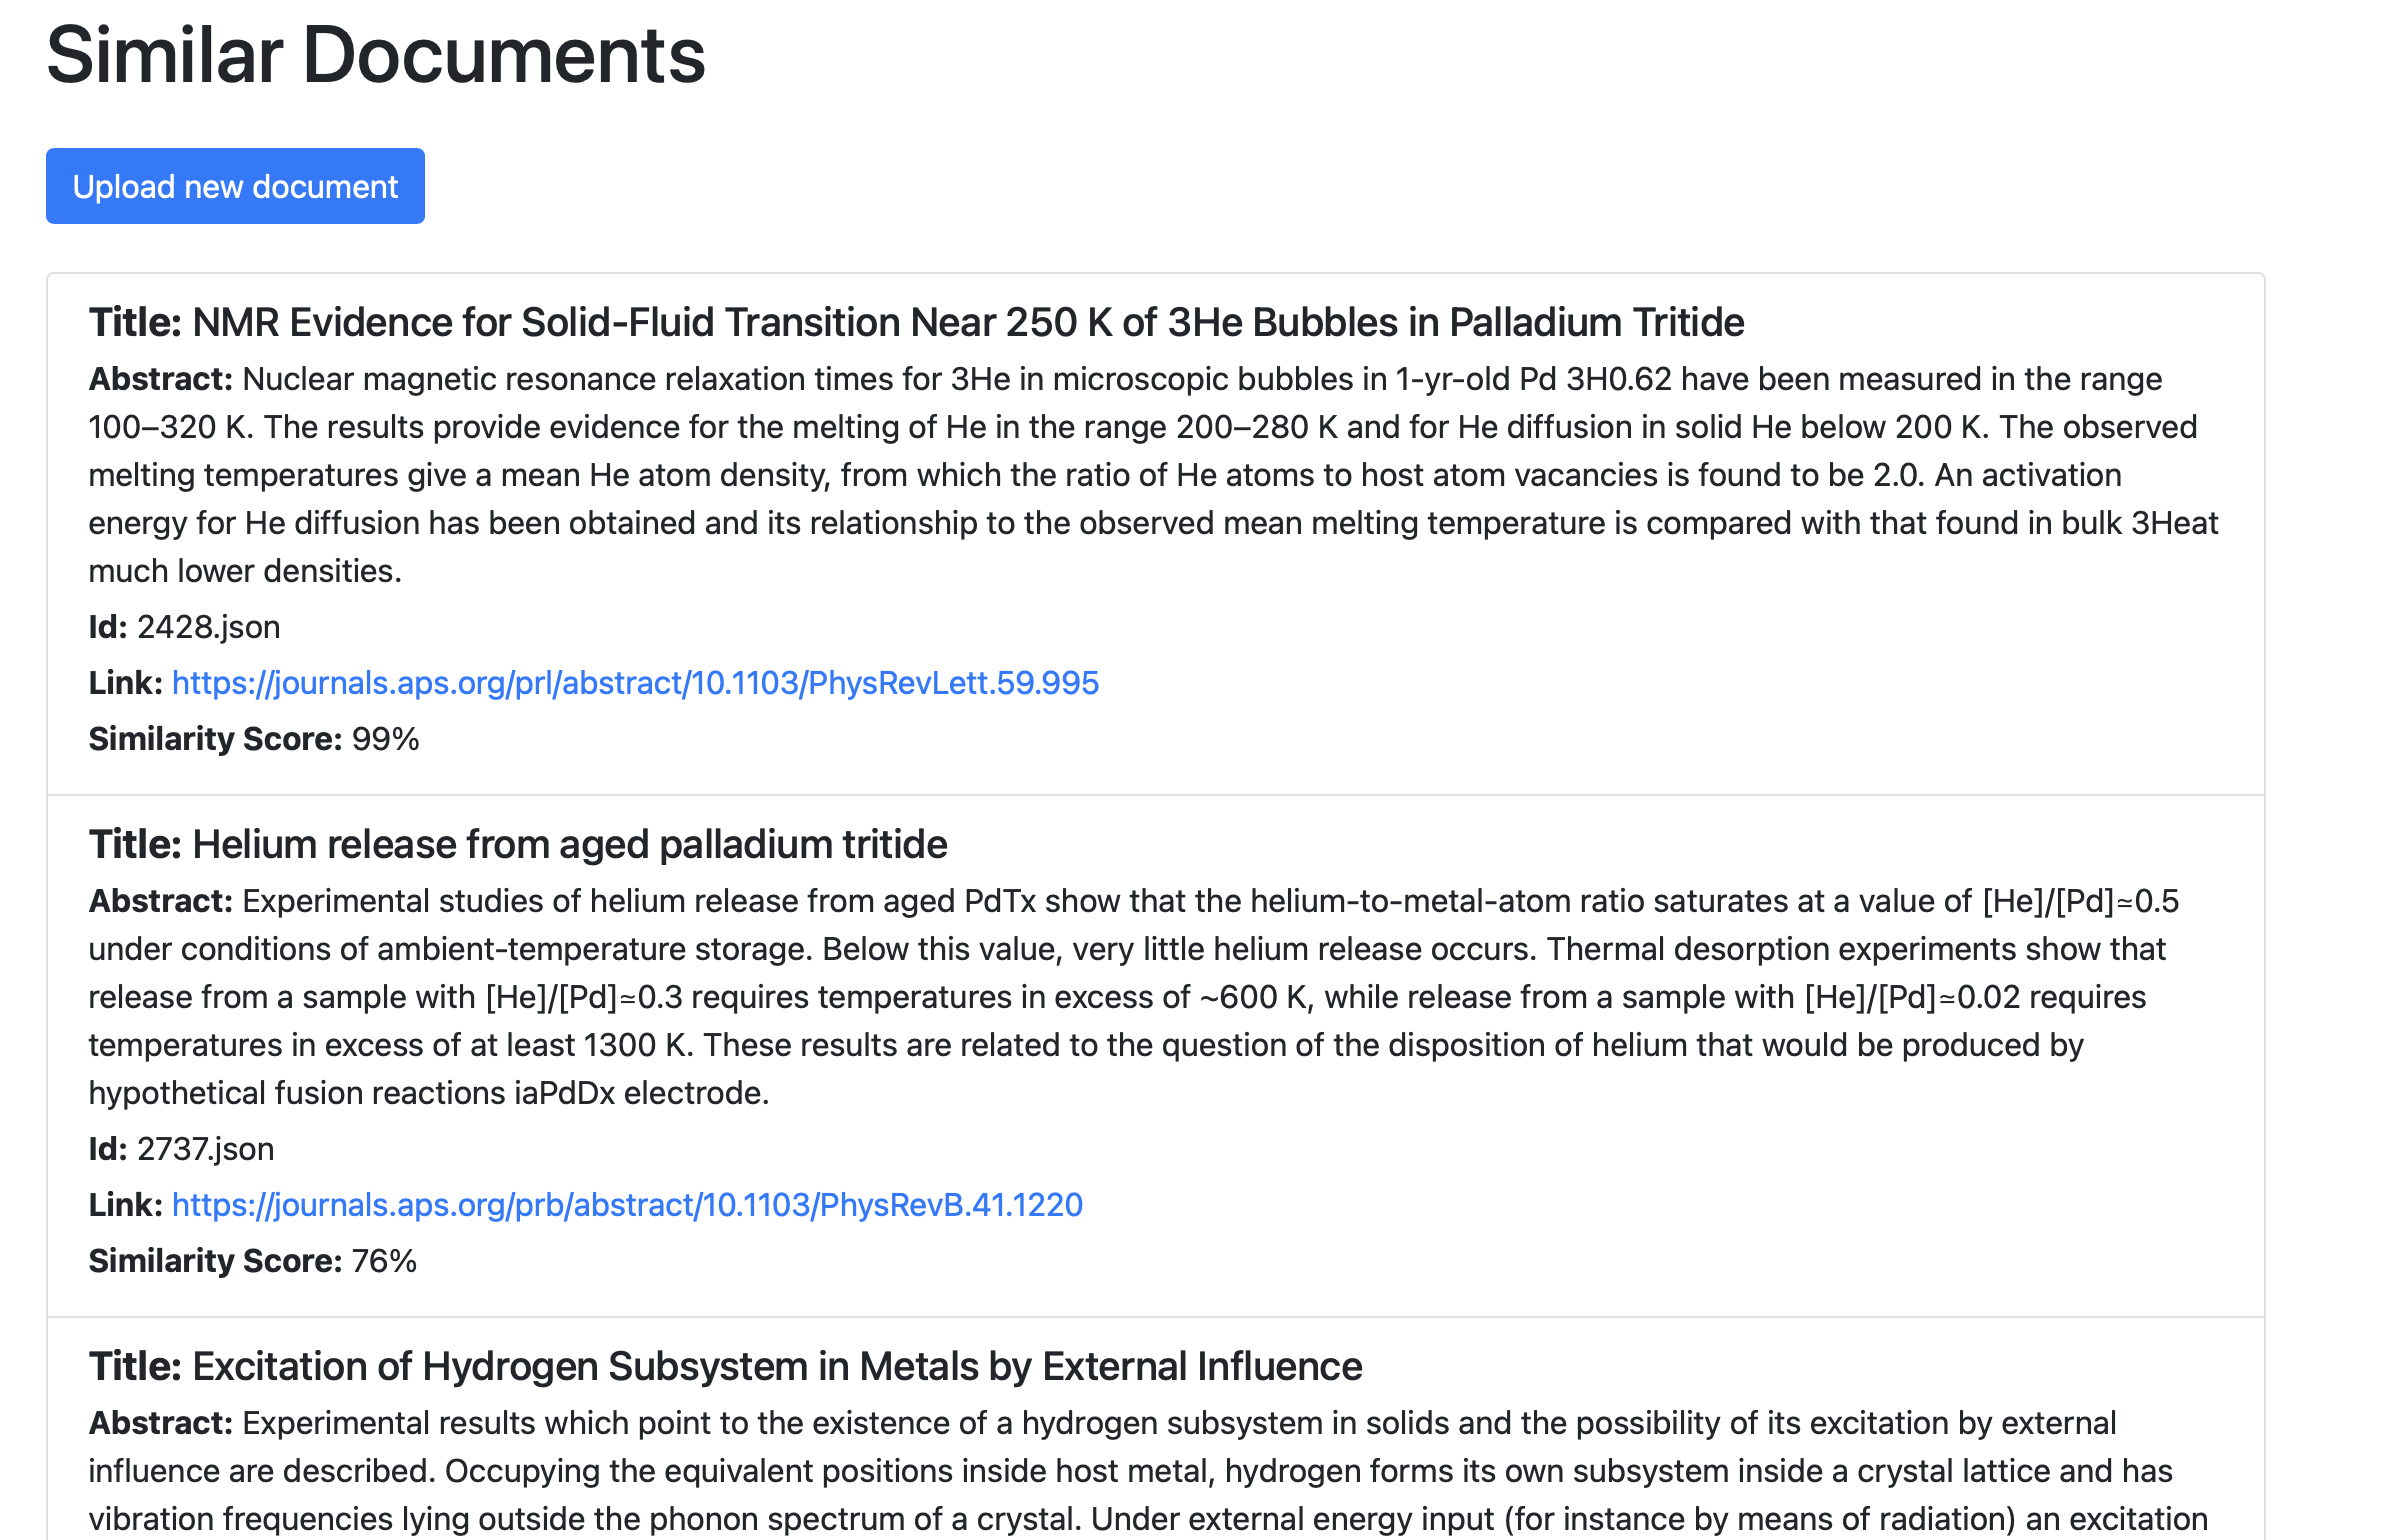
\includegraphics[width=0.8\textwidth]{images/result.png}
        \caption{Screenshot of the results page}
        \label{fig:Screenshot of the results page}
    \end{figure}

\section{Conclusion}
    This study demonstrates the potential of AI techniques, particularly topic modeling and document similarity algorithms, to advance research in LENR. The results will help researchers navigate and synthesize the vast body of LENR literature, fostering new discoveries and accelerating innovation in the field.

\section{References}
\begin{itemize}
    \item Fan, L., Li, L., et al. (2023). "A bibliometric review of large language models research from 2017 to 2023." arXiv. doi: 10.48550/arXiv.2304.02020.
    \item Blei, D. M., Ng, A. Y., and Jordan, M. I. (2003). "Latent Dirichlet Allocation." J. Mach. Learn. Res. 3, 993–1022.
    \item Grootendorst, M. (2022). "BERTopic: Neural topic modeling with a class-based TF-IDF procedure." arXiv. doi: 10.48550/arXiv.2203.05794.
\end{itemize}
\end{document}
